\documentclass{article}
\usepackage[letterpaper,margin=1in]{geometry}
\usepackage{amsmath}
\newcounter{magicrownumbers}
\newcommand\rownumber{\stepcounter{magicrownumbers}\arabic{magicrownumbers}}
\setcounter{magicrownumbers}{99}
\usepackage{multicol}
\usepackage{tikz}
\usetikzlibrary{automata,arrows,positioning,calc}
\usepackage{listings}
\renewcommand{\thepart}{\Roman{part}}
%\renewcommand{\thesection}{\arabic{section}.}\\
\renewcommand{\thesection}{\arabic{section}.}
\renewcommand{\thesubsection}{\arabic{subsection}.}
%\renewcommand{\thesubsection}{\alph{subsection})}
\usepackage[numbered,framed]{matlab-prettifier}
\usepackage{enumerate}
\usepackage{hyperref}
\usepackage{chngcntr}
\counterwithin*{section}{part}
\usepackage{color}
\usepackage{pgfplots}

\begin{document}
	\null\hfill\begin{tabular}[t]{l@{}}
	Matteson Daniel-Padgett, Lena Tan\\
	999096167, 999098385\\
	December 8, 2017\\
	ECS 152A
\end{tabular}
	
\begin{center}	
\sc \Large Project 2
\end{center}	

\part{}	
	
\section{}
Simple queue system model:$\mu = 1$ \\
\begin{center}
\begin{tabular}{c | c | c | c | c | c | c | c}
	Lambda & Count & Min & Max & Mean & Median & Sd & Utilization \\
	\hline
	0.200 & 200377 & 0.000 & 15.023 & 1.251 & 0.867 & 1.254 & 0.200 \\ 
	0.400 & 400070 & 0.000 & 18.180 & 1.658 & 1.146 & 1.660 & 0.399 \\ 
	0.600 & 601173 & 0.000 & 30.204 & 2.529 & 1.749 & 2.539 & 0.603 \\ 
	0.800 & 799713 & 0.000 & 54.270 & 4.996 & 3.452 & 4.988 & 0.800 \\ 
	0.900 & 898679 & 0.000 & 90.886 & 9.558 & 6.698 & 9.370 & 0.897 \\
	0.990 & 991142 & 0.000 & 419.359 & 86.938 & 64.409 & 76.626 & 0.990 \\
\end{tabular} \\
\end{center}

\section{}
	\begin{center}
	   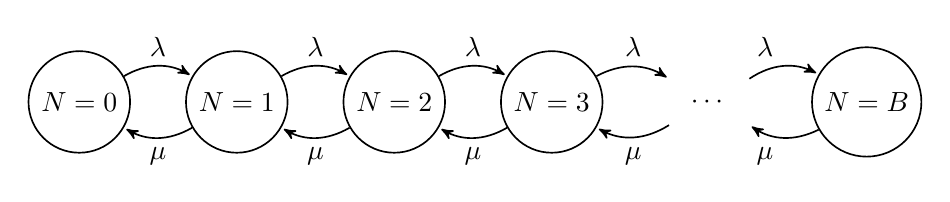
\begin{tikzpicture}[->,>=stealth',shorten >=1pt,auto,node distance=2cm,semithick]
		  \tikzstyle{every state}=[fill=white,draw=black,text=black,minimum size=1.1cm]
		
		  \node[state] (A) {$N=0$};
		  \node[state] (B) [right of=A] {$N=1$};
		  \node[state] (C) [right of=B] {$N=2$};
		  \node[state] (D) [right of=C] {$N=3$};
		  \node[minimum size=1cm] (E) [right of=D] {$\cdots$};
		  \node[state] (F) [right of=E] {$N=B$};
		
		  \path (A) edge [bend left] node {$\lambda$} (B);
		  \path (B) edge [bend left] node {$\mu$} (A);
		  \path (B) edge [bend left] node {$\lambda$} (C);
		  \path (C) edge [bend left] node {$\mu$} (B);
		  \path (C) edge [bend left] node {$\lambda$} (D);
		  \path (D) edge [bend left] node {$\mu$} (C);
		  \path (D) edge [bend left] node {$\lambda$} (E);
		  \path (E) edge [bend left] node {$\mu$} (D);
		  \path (E) edge [bend left] node {$\lambda$} (F);
  		  \path (F) edge [bend left] node {$\mu$} (E);
		\end{tikzpicture}
	\end{center}
    Let $P(N) = \pi_N$ denote the probability that there are $N$ packets in the queue. Applying flow balance gives: 
    $$\pi_0\lambda = \pi_1\mu \xrightarrow{} \pi_1 = \frac{\lambda}{\mu}\pi_0$$
    $$\pi_1(\lambda + \mu) = \pi_0\lambda + \pi_2\mu \xrightarrow{} \pi_2 = (\frac{\lambda}{\mu})^2\pi_0$$
    $$\pi_N = (\frac{\lambda}{\mu})^N\pi_0$$
    The sum of the probabilities at each state must equal one such that
    $$\pi_0 = 1 - \sum_{N=1}^{B}\pi_N = 1 - \pi_0\sum_{N=1}^{B}(\frac{\lambda}{\mu})^N = \frac{1}{\sum_{N=0}^{B}(\frac{\lambda}{\mu})^N}$$
    Simplifying,
    $$\pi_N = \frac{(\frac{\lambda}{\mu})^N}{\sum_{N=0}^{B}(\frac{\lambda}{\mu})^N}$$
    Packet loss occurs when the buffer is full and a packet arrives, so the packet loss probability $P_d$ is determined by $$\lambda P(N=B) = \lambda \frac{(\frac{\lambda}{\mu})^B}{\sum_{N=0}^{B}(\frac{\lambda}{\mu})^N}$$

\section{}
\begin{center}
\begin{tabular}{c | c | c | c | c | c | c | c | c | c | c}
	B         & Lambda    & Count     & Min       & Max       & Mean      & Median    & Sd        & Utilization & Dropped   & $P_d$     \\
	\hline
	10        & 0.200     & 200377    & 0.000     & 15.023    & 1.251     & 0.867     & 1.254     & 0.200     & 0         & 0.000     \\
	10        & 0.400     & 401172    & 0.000     & 23.096    & 1.664     & 1.154     & 1.660     & 0.402     & 23        & 0.000     \\
	10        & 0.600     & 599482    & 0.000     & 24.461    & 2.455     & 1.730     & 2.375     & 0.601     & 1518      & 0.003     \\
	10        & 0.800     & 781331    & 0.000     & 30.045    & 3.790     & 2.954     & 3.200     & 0.781     & 18248     & 0.023     \\
	10        & 0.900     & 854259    & 0.000     & 32.460    & 4.640     & 3.931     & 3.528     & 0.854     & 45830     & 0.054     \\
	10        & 0.990     & 905912    & 0.000     & 27.556    & 5.389     & 4.887     & 3.687     & 0.904     & 84557     & 0.093     \\
	50        & 0.200     & 199916    & 0.000     & 14.758    & 1.241     & 0.859     & 1.244     & 0.199     & 0         & 0.000     \\
	50        & 0.400     & 400067    & 0.000     & 26.712    & 1.664     & 1.152     & 1.666     & 0.399     & 0         & 0.000     \\
	50        & 0.600     & 599600    & 0.000     & 30.476    & 2.491     & 1.733     & 2.477     & 0.599     & 0         & 0.000     \\
	50        & 0.800     & 801180    & 0.000     & 48.397    & 4.976     & 3.456     & 4.933     & 0.801     & 0         & 0.000     \\
	50        & 0.900     & 898139    & 0.000     & 68.222    & 9.539     & 6.721     & 9.105     & 0.897     & 334       & 0.000     \\
	50        & 0.990     & 974218    & 0.000     & 79.242    & 23.823    & 22.600    & 15.271    & 0.975     & 16028     & 0.016     \\
\end{tabular} \\
\end{center}

\section{}
\begin{center}
\begin{tabular}{c | c | c | c}
    B   & Lambda  & Simulation $P_d$    & Theoretical $P_d$ \\
    \hline
    10  & 0.200   & 0.000   & 0.000 \\
    10  & 0.400   & 0.000   & 0.000 \\
    10  & 0.600   & 0.003   & 0.002 \\ 
    10  & 0.800   & 0.023   & 0.023 \\
    10  & 0.900   & 0.054   & 0.051 \\
    10  & 0.990   & 0.093   & 0.086 \\
    50  & 0.200   & 0.000   & 0.000 \\
    50  & 0.400   & 0.000   & 0.000 \\
    50  & 0.600   & 0.000   & 0.000 \\
    50  & 0.800   & 0.000   & 0.000 \\
    50  & 0.900   & 0.000   & 0.001 \\
    50  & 0.990   & 0.016   & 0.015 \\
\end{tabular}
\end{center}
As shown by the table above, the simulation packet loss probability closely follows the theoretical packet loss probability.

\part{}	
\section*{Hand Simulation}
\begin{center}
\begin{tabular}{| c | c | c | c | c | c | c | c | c | c |}
	\hline
    Timestep & \multicolumn{3}{|c|}{Node 1} & \multicolumn{3}{|c|}{Node 2} & \multicolumn{3}{|c|}{Node 3} \\
    \cline{2-10}
      & L & S & N & L & S & N & L & S & N \\
    \hline
    \rownumber & 2 & 100 & 0 & 3 & 100 & 0 & 2 & 100 & 0 \\
    \hline
    \rownumber &  &  &  &  &  &  &  &  &  \\
    \hline
\end{tabular}
\end{center}
	
\section*{Exponential}
\begin{center}
\includegraphics[width=1\linewidth]{Exponential_plot}
\begin{tabular}{c | c | c | c}
	Lambda    & Total Time Slots & Successful Transmissions & Throughput \\
	\hline
	0.010     & 100000    & 9912      & 0.099     \\
	0.020     & 100000    & 19945     & 0.199     \\
	0.030     & 100000    & 29811     & 0.298     \\
	0.040     & 100000    & 39976     & 0.400     \\
	0.050     & 100000    & 49616     & 0.496     \\
	0.060     & 100000    & 59379     & 0.594     \\
	0.070     & 100000    & 68745     & 0.687     \\
	0.080     & 100000    & 76704     & 0.767     \\
	0.090     & 100000    & 81354     & 0.814     \\
\end{tabular} \\
\end{center}

\section*{Linear}
\begin{center}
\includegraphics[width=1\linewidth]{Linear_plot}
\begin{tabular}{c | c | c | c}
	Lambda    & Total Time Slots & Successful Transmissions & Throughput \\
	\hline
	0.010     & 100000    & 9969      & 0.100     \\
	0.020     & 100000    & 19953     & 0.200     \\
	0.030     & 100000    & 28246     & 0.282     \\
	0.040     & 100000    & 28851     & 0.289     \\
	0.050     & 100000    & 29143     & 0.291     \\
	0.060     & 100000    & 28670     & 0.287     \\
	0.070     & 100000    & 28978     & 0.290     \\
	0.080     & 100000    & 29153     & 0.292     \\
	0.090     & 100000    & 28823     & 0.288     \\
\end{tabular} \\
\end{center}

\section*{Exponential vs. Linear}
\begin{center}
\includegraphics[width=1\linewidth]{Exponential_Linear_plot}
\end{center}

\end{document}
\grid
\grid
